\section{Project Setup}
\label{sec:setup}
The model car consists of the following components: 

\begin{itemize}
    \item Servos: In total there are three servos for the brakes, one servo for steering and an engine for acceleration placed on the model car. All of these components can be controlled via a servo controller board.
   
    \item Servo Controller Board: The servo controller board is a \textit{pololu maestro mini servo controller board} which is attached to a Raspberry Pi via a usb-to-uart bridge. The braking servos and the steering servo, respectively are connected to the board, whereas the engine can not be controlled with it for several reasons.
   
    \item Raspberry Pi: The Raspberry Pi is responsible for sending control commands to the servo controller board. It receives its input data from a PandaBoard via a mqtt topic to which it is subscribed. The Raspberry Pi runs Genode with Fiasco.OC.
   
    \item PandaBoard: Besides the Raspberry Pi, the PandaBoard is the second ECU in the model car. It also runs Genode with Fiasco.OC. The task is to receive data from a simulation, transform the data into concrete servo values and send them via mqtt to the Raspberry Pi.
\end{itemize}

An image of the model car is shown in figure \ref{fig:model}. The servos can be seen in box a. Box b shows the Raspberry Pi. The PandaBoard is placed on top of the car and can be seen in box c. The servo controller board is placed behind the Raspberry Pi which can not be seen in the image. All of the mentioned components are described in more detail in chapter~\ref{sec:arch}. \\

\begin{figure}[h]
       \centering
       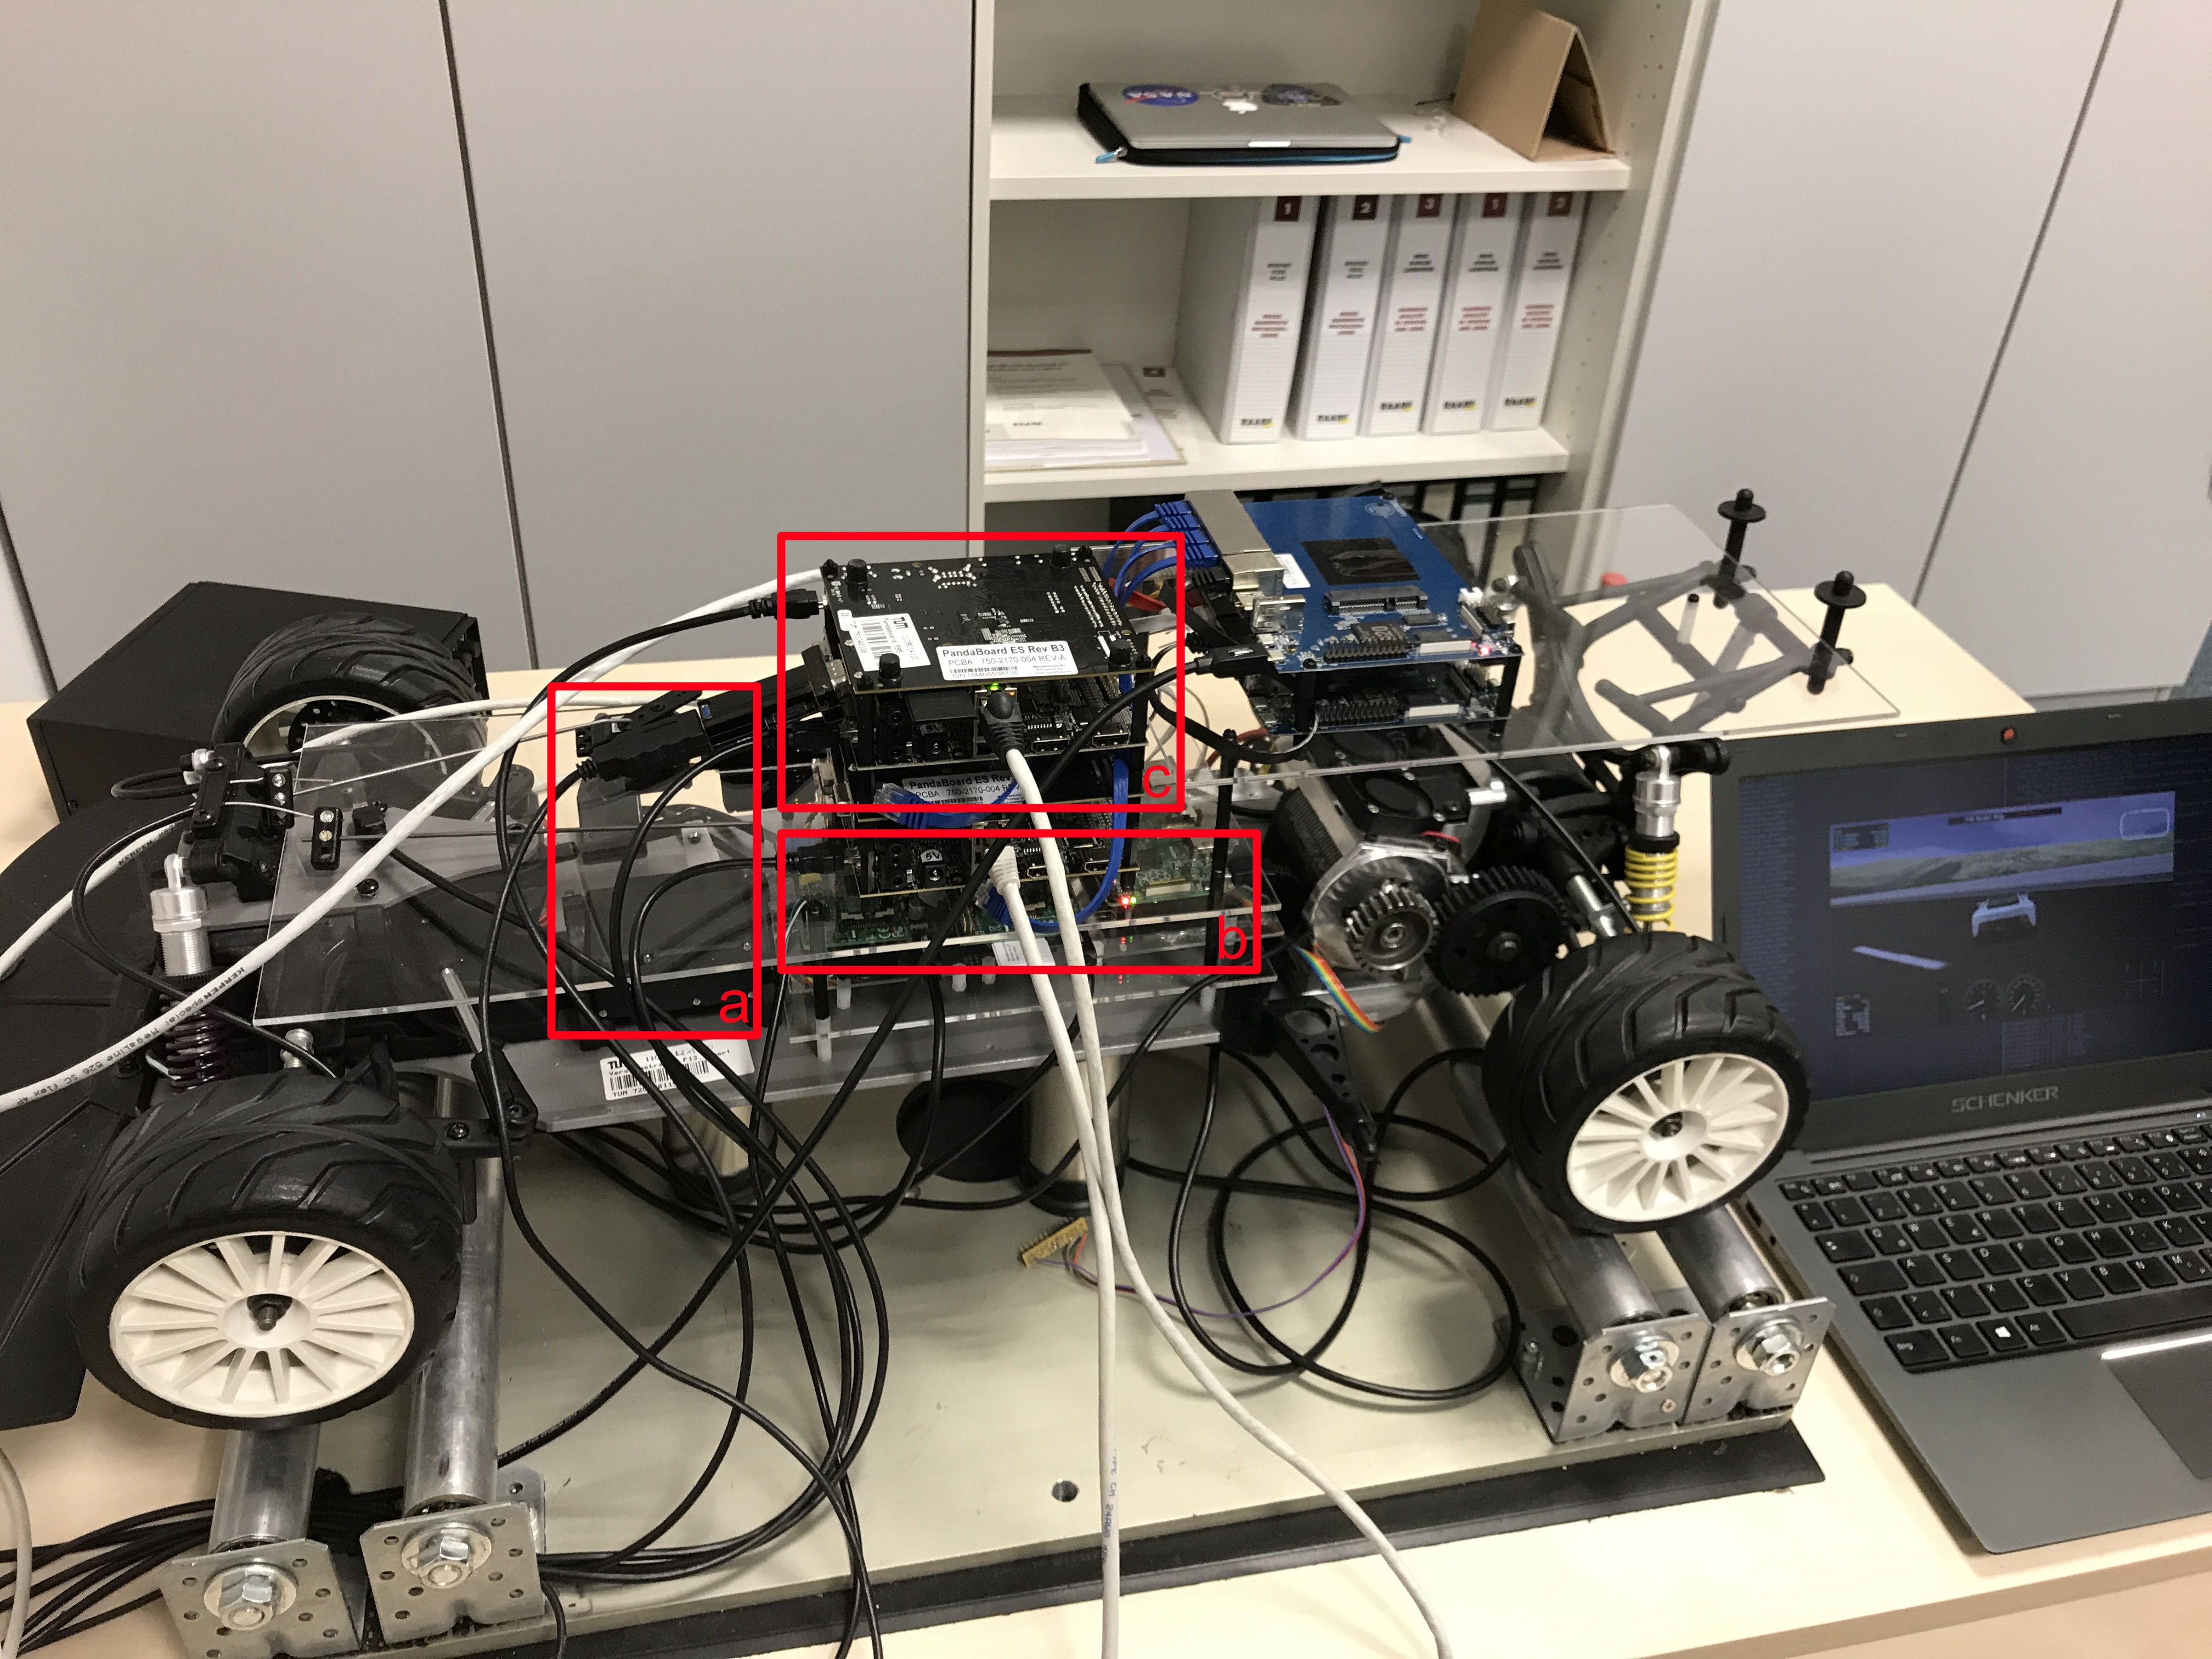
\includegraphics[trim={0 10cm 0 30cm},clip,width=1.0\linewidth]{images/model}
       \caption{Model Car}
       \label{fig:model}
\end{figure}




%%%%%%%%%%%%%%%%%%%%%%%%%%%%%%%%%%%%%%%%%%%%%%%%%%%%%%%%%%%%
\section{Source Code Structure}
\label{sec:scs}
The complete structure of the project directory is illustrated in figure \ref{fig:structure}. All of the subdirectories are described in more detail in the following chapter.
For integration in the argos-research build environment it is expected that this repository is placed in the \texttt{genode/repos/} directory of the \texttt{argos-research/operating-system} repository. \\

\begin{figure}[h]
    \dirtree{%
    .1 car\_project.
    .2 run.
    .2 include.
    .3 servo\_session.
    .3 controller\_session.
    .2 src.
    .3 mqtt.
    .3 rpi\_component.
    .4 rpi.
    .4 servo.
    .3 panda\_component.
    .4 panda.
    .4 controller.
    .2 old.
    .3 linux.
    .3 pololu.
    }
    \caption{Structure of the project directory}
    \label{fig:structure}
\end{figure}


\paragraph{run}
The run folder contains the run files for the PandaBoard (\texttt{car\_panda.run}) and the Raspberry Pi (\texttt{car\_rpi.run}).
These files are responsible for defining the project build components and the boot modules. Additionally, they contain the configuration for the started modules.

\paragraph{include}
In the include directory the header files for the servo component (\texttt{servo\_session}) and the controller component (\texttt{controller\_session}) are split up into their respective folders.

\paragraph{include/servo\_session}
Contains all the header files for the servo component that is part of the Genode application running on the Raspberry Pi. Ihe interface is described in section~\ref{sec:comp-servo}.

\paragraph{include/controller\_session}
Contains all the header files for the controller component that is part of the Genode application running on the PandaBoard. The interface is described in section~\ref{sec:comp-controller}.

\paragraph{src}
The source directory contains all the source files of the project.
The different parts of the source code are split up into its own subfolders which are \texttt{mqtt}, \texttt{rpi\_component} and \texttt{panda\_component}.

\paragraph{src/mqtt}
Contains the header and the source file of the mqtt client. The client implements the mosquitto interface and is used in both, the \texttt{panda\_component} and the \texttt{rpi\_component}.

\paragraph{src/rpi\_component}
Contains the code for the Genode application running on the Raspberry Pi. It consists of two components which are placed in different subfolders. The functionality is described in detail in section \ref{sec:pi-genode}.

\paragraph{src/rpi\_component/rpi}
The rpi component is responsible for handling the commands received from the mqtt server and forwarding them to the servo component.

\paragraph{src/rpi\_component/servo}
The servo component controls the servos by sending commands over the serial connection to the pololu servo controller board.

\paragraph{src/panda\_component}
Contains the code for the Genode application running on the PandaBoard. It consists of two components which are placed in different subfolders. The functionality is described in detail in section \ref{sec:panda-genode}.

\paragraph{src/panda\_component/panda}
The panda component sets up the network and uses the mqtt class to connect to the mqtt server during initialization. Afterwards, it passes on the \texttt{car-control} topic received commands to the controller component and publishes the result on the \texttt{car-servo} topic.

\paragraph{src/panda\_component/controller}
The controller component transforms abstract commands from the simulation to pwm values.

\paragraph{old}
The old folder contains programs and scripts used during development.

\paragraph{old/linux}
An implementation of the rpi and panda components as linux user programs can be found in the \texttt{linux} folder.
These were used for development during the first phase of the project when the rpi Genode image has not been available yet.

\paragraph{old/pololu}
In the subdirectory pololu resides a shell script and a c-program, which are originally from the pololu homepage and can be used for hardware testing.

\newpage
%%%%%%%%%%%%%%%%%%%%%%%%%%%%%%%%%%%%%%%%%%%%%%%%%%%%%%%%%%%%
\section{Application Programming Interfaces}
\label{sec:api}

%%%%%%%%%%%%%%%%%%%%%%%%%%%%%%%%%%%%%%%%%%%%%%%%%%%%%%%%%%%%
\subsection{Mqtt client}
We use mqtt for both, the communication between the simulation and the PandaBoard and the communication between the PandaBoard and the Raspberry Pi. The implementation of the mqtt client is based on the mosquitto library which is already ported for Genode. The client is able to publish messages on a specified topic or receive messages from a topic to which it is subscribed. 

\subsubsection{car-control}
\label{sec:mqtt-car-control}
\texttt{car-control} is the topic name of the mqtt topic to which the PandaBoard is subscribed to. Commands to this topic are sent from the simulation. All commands need to have the following format: \\

\textbf{Format:} (command,value) \\
Command describes the type of request, i.e. braking, steering or acceleration. Value describes the strength of the command. All commands and values are listed in table \ref{tab:car-control}.

\textbf{Example:} (1,0.5) \\
This is a brake request with half braking force.

\begin{table}[h]
    \centering
    \begin{tabular}{c | c | c}
        \textbf{Command} & \textbf{Value Range} & \textbf{Meaning} \\ \hline
        0   &   [ -1.0 ; 1.0 ]    & Steering \\
        1   &   [ 0 ; 1.0 ]       & Brake \\ 
        2   &   [ 0 ; 1.0 ]       & Acceleration \\ 
    \end{tabular}
    \caption{Allowed values for the car-control topic}
    \label{tab:car-control}
\end{table}


\subsubsection{car-servo}
\label{sec:mqtt-car-servo}
\texttt{car-servo} is the topic name of the mqtt topic to which the Raspberry Pi is subscribed to. Commands to this topic are sent from the PandaBoard. All commands need to have the following format: \\ 

\textbf{Format:} (channel,value) \\
Channel is a number ranging from 0 to 11 and describes the channel number on the servo controller board. The braking servos are connected to channels 0, 1 and 2, whereas the steering servo is connected to channel 6. Values are pwm signals ranging from 4500 to 7500. The neutral value for the servo is 6000. The main engine can not be controlled with the pololu maestro servo controller board.

\textbf{Example:} (0,7500) \\
This command sends a pwm signal with value 7000 to channel 0. This means that the brake connected to channel 0 gets activated with full force. 




%%%%%%%%%%%%%%%%%%%%%%%%%%%%%%%%%%%%%%%%%%%%%%%%%%%%%%%%%%%%
\subsection{Servo component}
\label{sec:comp-servo}

The servo component provides five methods. All methods return -1 in case of an error, else 0. Obviously, the getter functions return the requested value.
\autoref{lst:servo} shows the corresponding function declarations exported to Genode.
\begin{itemize}
\item The function \textbf{setTarget} receives the channel of the connected servo and the target position as parameters.
\item The function \textbf{setSpeed} receives the channel of the connected servo and the maximum speed of the servo as parameters. A value of 0 means unlimited.
\item The function \textbf{setAcceleration} receives the channel of the connected servo and the maximum acceleration of the servo as parameters. A value of 0 means unlimited.
\item The function \textbf{getPosition} receives the channel of the connected servo and returns its current position.
\item The function \textbf{getMovingState} returns 0 if no servo is currently moving, else 1.
\end{itemize}

\begin{lstlisting}[language=c, frame=single, basicstyle=\footnotesize,  label={lst:servo}, caption=Genode interface for servo component]
GENODE_RPC(Rpc_setTarget, int, setTarget, unsigned char, unsigned short);
GENODE_RPC(Rpc_setSpeed, int, setSpeed, unsigned char, unsigned short);
GENODE_RPC(Rpc_setAcceleration, int, setAcceleration, unsigned char, 
						      unsigned short);
GENODE_RPC(Rpc_getPosition, int, getPosition, unsigned char);
GENODE_RPC(Rpc_getMovingState, int, getMovingState);
\end{lstlisting}



\subsection{Controller component}
\label{sec:comp-controller}

The controller component provides two methods each expecting a double as input and returning an integer value.
\autoref{lst:servo} shows the corresponding function declarations exported to Genode.
\begin{itemize}
\item The function \textbf{transform\_steer} transforms a steering angle between -1 and 1 where -1 is completely right, and returns the corresponding pwm value in quarter microseconds for the servo.
\item The function \textbf{transform\_brake} transforms a braking value between 0 and 1 where 1 means fully applied, and returns the corresponding pwm value in quarter microseconds for the servo.
\end{itemize}

\begin{lstlisting}[language=c, frame=single, basicstyle=\footnotesize,  label={lst:controller}, caption=Genode interface for controller component]
GENODE_RPC(Rpc_transform_steer, int, transform_steer, double);
GENODE_RPC(Rpc_transform_brake, int, transform_brake, double);
\end{lstlisting}
